\clearpage
\section{Additional Processing Diagnostics}
Figure~\ref{fig:supp-diagnostics} retains the complete breakdown of the 1,024 evaluation station--file records. The three panels summarize the same records by different groupings; their counts must not be added across panels. Source-file sensing blocks in panel (c) differ from the center-pixel reporting blocks used for valid opportunities in the main station--block matrix.

\begin{figure}[htbp]
\centering
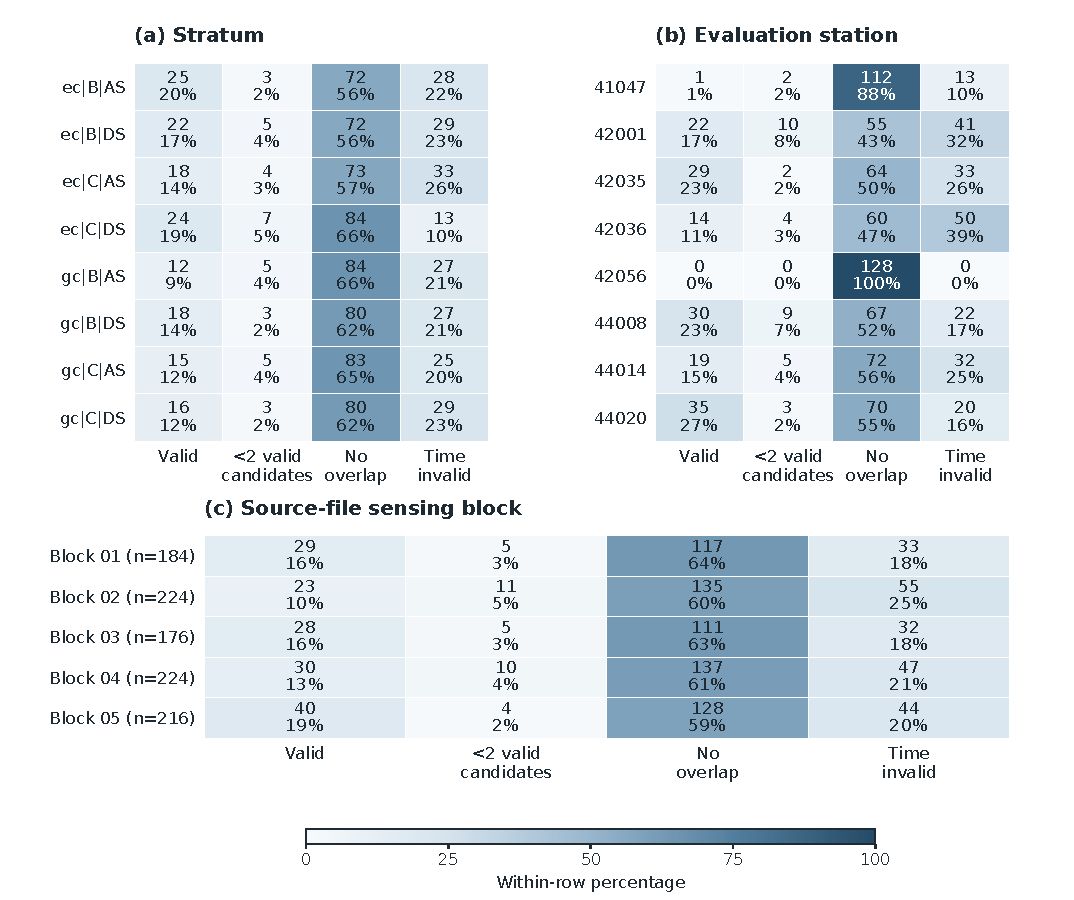
\includegraphics[width=\textwidth]{../paper/figures/figure5.pdf}
\caption{Evaluation processing states by (a) sector--platform--pass stratum, (b) station, and (c) source-file sensing block. In (a), ec/gc denote the Atlantic/Gulf product sectors, B/C denote MetOp-B/MetOp-C, and AS/DS denote ascending/descending passes. Cells show counts and within-row percentages. Each row in (a) and (b) has 128 records; the block denominators in (c) differ. All records in panel (c) are grouped by file sensing time, because failed records lack a valid center-pixel time. These are descriptive processing categories, not causal diagnoses.}
\label{fig:supp-diagnostics}
\end{figure}
